\section{The effect of linked selection on patterns of neutral diversity}

A newly derived allele with an additive selection coefficient $s$ will
take a time $\tau \approx 4\log(2N)/s$ generations to reach to fixation
within our population (see eqn. \eqref{eq:diploid_fix_time}). This short time window offers very little time
for recombination between the selected site and linked neutral
sites.  \\

First lets imagine examining variation at a locus fully linked
to our selected locus, just after our sweep reached fixation. A pair of neutral alleles sampled at this locus
must both trace their ancestral lineages back through to the neutral
allele on whose background the selected allele initially arose. As
that neutral allele, which existed $\tau$ generations ago is the
ancestor of the entire population at this locus. Our individuals who
carry the beneficial allele are, from the perspective of these two
alleles, exactly like a rapidly expanding population. Therefore, our
pair of neutral alleles sampled at our locus will be forced to
coalesce $\approx \tau$ generations ago. This is a very
short-time scale compared to the average neutral coalescent tie of
$2N$ generations of a pair of alleles.\\

If we now allow recombination into our model we can think about a pair
of alleles sampled at a neutral locus a recombination distance $r$
away from our selected site. Our pair of alleles will be forced to
coalesce $\approx \tau$ generations if neither of them reside on
haplotypes that the selected allele recombined onto during the
sweep. This is equivalent to saying that neither of our neutral
alleles recombine off of the beneficial allele's background moving
backward in time.\\

The probability that our lineage fail recombines off our beneficial
allele's background and onto the
ancestral background in the $j^{th}$ generation back is
\begin{equation}
r (1-X(j))
\end{equation}
so the probability ($p_{NR}$) that our lineage fails to recombine off in the
$\tau$ generations it takes our selected allele to move through the
population is
\begin{equation}
p_{NR}=\prod_{j=1}^{\tau} \big(1- r(1-X(j))\big)
\end{equation}
assuming that $r$ is small then $ \left(1- r(1-X(j))\right) \approx
e^{-r(1-X(j))}$, such that
\begin{equation}
p_{NR}=\prod_{j=1}^{\tau} \left(1- r(1-X(j))\right) \approx \exp
\left( -r\sum_{j=1}^{\tau}
1- X(j) \right) =\exp
\left( -r \tau (1-\widehat{X}) \right)
\end{equation}
where
$\widehat{X}$ is the average frequency of the derived allele across the trajectory
$\widehat{X} = \frac{1}{\tau}  \sum_{j=1}^{\tau}
 X(j)$. As our allele is additive its trajectory for frequencies
 $<0.5$ is the mirror image of its trajectory for frequency $>0.5$, therefore it
average frequency $\widehat{X} =0.5$. So
\begin{equation}
p_{NR} = e^{-r \tau/2 }.
\end{equation}
The probability that both of our lineages fail to recombine off the
sweep and hence are forced to coalesce is $p_{NR}^2$, assuming that
they coalesce at a time close to $\tau$ so that they recombine
independently of each other for times $< \tau$.\\

If one or other of our lineages recombine off the sweep it will take them on average
$\approx 2N$ generations to find a common ancestor as we are back our
neutral coalescent. Thus the expected time
till our pair of lineages find a common ancestor is
\begin{equation}
\E(T_2)  = \tau \times p_{NR}^2 +(1-p_{NR}^2) (\tau +2N) \approx
\left(1-p_{NR}^2 \right) 2N
\end{equation}
where this last approximation assumes that $\tau \ll 2N$. So the
expected pairwise diversity for neutral alleles at a recombination
distance $r$ away from the selected sweep  ($\pi_r$) is
\begin{equation}
\E(\pi_r) = 2\mu \E(T_2)  \approx \theta \left(1-e^{-r\tau} \right) \label{eqn:pi_HH}
\end{equation}
so diversity increases as we move away from the selected site,
slowly exponentially plauteuing to its neutral expectation $\theta=4N\mu$.\\

To get a sense of the physical scale over which diversity is reduced
consider a region where recombination occurs at a rate $r_{BP}$ per
base pair per generation, and our locus is $ \ell $ base pairs away from the
selected site $r=r_{BP } \ell $ (where $r_{BP}  \ell  \ll 1$ so we don't need to
worry about more than one recombination event occurring per
generation). Typical
recombination rates are on the order of $r_{BP} = 10^{-8}$, in Figure
\ref{fig:hitchhiking_reduction} we show the reduction in diversity,
given by eqn. \eqref{eqn:pi_HH}, for two different selection coefficients.\\ 

For our expected diversity levels to recover to $50\%$ of
its neutral expectation $\E(\pi_r)/\theta=0.5$, requires a physical
distance $\ell^{*}$ such that $\log(0.5) = -r_{BP} \ell ^*\tau$ as using our
expression for $\tau$ then $ \ell^* = \frac{-\log(0.5)}{r_{BP} \tau }$. As
$\tau$ depends inversely on the selection $s$ (eqn. \eqref{eq:diploid_fix_time}), the width of our trough of reduced diversity depends on $s/r_{BP}$.
All else being equal we expect stronger sweeps or sweeps in regions of low
recombination to have a larger hitchhiking effect. So that a selection coefficient of $s=0.1\%$ would reduce
diversity over 10's of kb, while a sweep of $s=1\%$ would affect
$\sim$100kb.   \\


\begin{figure}
\begin{center}
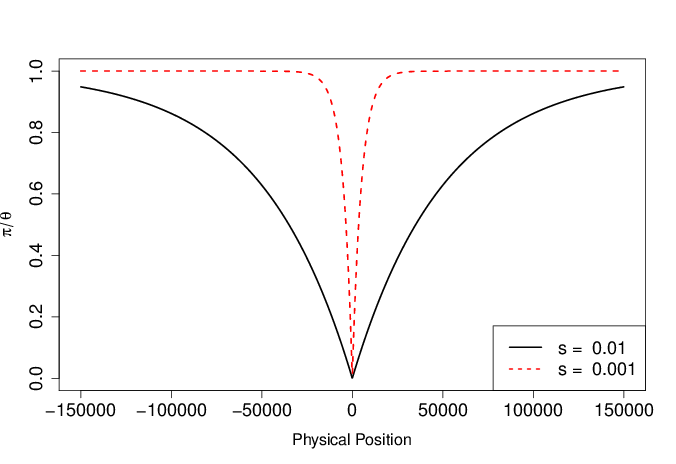
\includegraphics[width=0.5\textwidth]{figures/hitchhiking_reduction.png}
\end{center}
\caption{Reduction in diversity compared to its neutral expectation as
a function of the distance away from a site where a selected allele
has just gone to fixation. The recombination rate is $r_{BP}= 1\times
10^{-8}$.} \label{fig:hitchhiking_reduction}
\end{figure}

\begin{question}
A recently published study has identified the genetic basis of
melanism in the pepper moth. This allele swept to fixation in northern
parts of the UK; a classic case of adaptation to industrial pollution
(made famous by the work of Kettlewell). The genetic basis of melanism
is a transposable element (TE) inserted into a pigmentation gene. The
investigators found that diversity is suppressed in a broad region
around the TE. Specifically, on the background of the TE, it takes
roughly 200 kb in either direction for diversity levels to recover to
50\% of genome-wide levels. \\

Random facts: In all moths and butterflies only males recombine;
chromosomes are transmitted without recombination in female. The
recombination rate in males is 2.9 cM/Mb.  Peppered moths have an
effective population size of roughly a hundred thousand
individuals. Kettlewell used to eat moths when out collecting them in
the field (personal communication, Art. Shapiro). \\
{\bf A)} Briefly explain how this pattern offers further evidence that the melanic allele was favoured by selection.\\
{\bf B)} Using this information what is your estimate as to the age of the allele?\\
{\bf C)} What is your estimate of the selection coefficient favouring this melanic?
\end{question}


\subsection{A simple recurrent model of selective sweeps}
We sample a pair of neutral alleles at a locus a genetic distance $r$ away from a locus where
sweeps are initiated within the population at some very low rate $\nu$
per generation. The waiting time between sweeps
at our locus is exponential $\sim Exp(\nu)$. Each sweep rapidly transits through the population in $\tau$
generations, such that each sweep is finished long before the next
sweep ($\tau \ll 1/\nu$). \\

As before our chance that our neutral lineage fails to recombine
off the sweep is $p_{NR}$, such that the probability that
our pair of lineages are forced to coalesce by a sweep $e^{-r \tau}$. Our
lineages therefore have a very low probability
\begin{equation}
\nu e^{-r \tau}
\end{equation}
of being forced to coalesce by a sweep per generation. In addition of
lineages can coalesce at a neutral rate of $1/(2N)$. Thus the average
waiting time till a coalescent event between our neutral pair of
lineages due to either a sweep or a neutral coalescent event is
\begin{equation}
\E(T_2) = \frac{1}{\nu e^{-r \tau} + 1/(2N)}
\end{equation}

Now imagine that the sweeps don't occur at a fixed location with
respect to our locus of interest, but now occur uniformly at random
across our sequence. The sweeps are initiated at a very low rate of
$\nu_{BP}$ per basepair per generation. The rate of coalescent due to
sweeps at a locus $\ell$ basepairs away from our neutral loci is
$\nu_{BP} e^{-r_{BP} \ell \tau}$. If our neutral locus is in the
middle of a chromosome that stretches $L$ basepairs in either direction
the total rate of sweeps per generation that force our pair of lineages to coalesce is
\begin{equation}
2\int_0^{L} \nu_{BP} e^{-r_{BP} \ell \tau} d \ell =
\frac{2\nu_{BP}}{r_{BP} \tau} \left(1-e^{-r_{BP} \tau L} \right)
\end{equation}
so that if $L$ is very large ($r_{BP} \tau L \gg 1$) the rate of coalesce per
generation due to sweeps is $\frac{2\nu_{BP}}{r_{BP} \tau}$. The total rate
of coalescence for a pair of lineages per generation is then
\begin{equation}
\frac{2\nu_{BP}}{r_{BP} \tau}+\frac{1}{2N}
\end{equation}
So our average time till a pair of lineages coalesce is
\begin{equation}
\E(T_2) = \frac{1}{\frac{2\nu_{BP}}{r_{BP} \tau}+\frac{1}{2N}} = \frac{r_{BP}2N}{\frac{4N\nu_{BP}}{ \tau}+r_{BP}}
\end{equation}
such that our expected pairwise diversity ($\pi=2\mu\E(T_2)$) in a region of
recombination rate $r_{BP}$ that experiences sweeps at rate $\nu_{BP}$
is  
\begin{equation}
\E(\pi) = \theta \frac{r_{BP}}{\frac{4N\nu_{BP}}{ \tau}+r_{BP}} \label{eqn:pi_GW_HH}
\end{equation}


\begin{figure}
\begin{center}
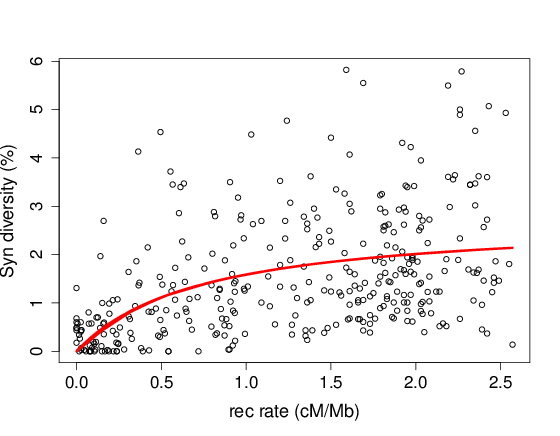
\includegraphics[width=0.5\textwidth]{figures/Genomewide_HH.png}
\end{center}
\caption{The relationship between (sex-averaged) recombination rate and synonymous
  site pairwise diversity ($\pi$) in {\it Drosophila melanogaster}
  using the data of Shapiro et al. 07 (kindly provided by Peter
  Andolfatto, see Sella et al. 09 for details). The curve is the
  predicted relationship between $\pi$ and recombination rate obtained
  by fitting equation \eqref{eqn:pi_GW_HH} to this data 
 using non-linear least squares via the {\tt nls()} function in {\tt R}.} \label{fig:GW_hitchhiking_reduction}
\end{figure}



